\intermediate{\subsection{Downloading the programs}}

\step{Downloading the programs.}{
    Download \texttt{BEAST} from \href{http://beast2.org}{\url{http://beast2.org}} and install it on your computer.
    This tutorial is written for the Mac OS X version of \texttt{BEAST} 2.4.5 or greater. Please make sure to keep \texttt{BEAST} and its packages up to date -- at the time of writing, the most recent version is 2.4.7.
    
    You will be using \texttt{BEAST} to run \texttt{SNAPP}, although it is possible to run \texttt{SNAPP} on its own. However, you 
    have to use \texttt{BEAST} in order to combine \texttt{SNAPP} and marginal likelihood estimation into the same analytical framework. 
    Thus, without \texttt{BEAST} you would not be able to conduct species delimitation with \texttt{SNAPP}.
    }

\step{Data included with the tutorial.}{
   After downloading and unzipping this archive you should have a ``BFD'' tutorial folder on your computer. This tutorial
    contains the files and folders shown in
    Box~\ref{box:tutorialDir}. The \menutab{data} folder contains the gecko SNP data in binary format (necessary for \texttt{SNAPP}). If you are unsure of how to convert your own
    SNP data from nucleotide to binary format, please read the documentation \href{http://beast2.org/tutorials/}{A rough guide to \texttt{SNAPP}} (Section 4. Preparing Input File). You can find scripts for converting SNP data into \texttt{SNAPP} input format at the phrynomics project site at \href{https://github.com/bbanbury/phrynomics}{GitHub}. You can also find help
    at the \texttt{BEAST} \href{https://groups.google.com/forum/?fromgroups\#!forum/beast-users}{Google users group}.
    The \menutab{xml} folder contains seven xml files (named according to the species delimitation models in Figure~\ref{fig:map}) that are ready to run in \texttt{BEAST}. 

    \begin{textbox}
        \centering
        \fbox{\begin{minipage}[c][15em][c]{0.5\textwidth}
            \ttfamily
            \begin{compactitem}
                \item BFD/
            \begin{compactitem}
                	\item BFD-tutorial.pdf
                    \item data/
                       \begin{compactitem}
                        \item hemi129.nex
                        \item smallhemi129.nex
                    \end{compactitem}
                    \item xml/
                    \begin{compactitem}
                        \item RunA.xml
                        \item RunB.xml
                        \item RunC.xml
                        \item RunD.xml
                        \item RunE.xml
                        \item RunF.xml
                        \item RunG.xml
                    \end{compactitem}
            \end{compactitem}
            \end{compactitem}
        \end{minipage}}
        \caption{The files included in this tutorial. The data folder contains the SNP data in binary format. Ready-to-run XML files are included in the xml folder.}
        \label{box:tutorialDir}
    \end{textbox}
}

\intermediate{\subsection{Setting up the XML file with \texttt{BEAUTi}}}

\step{Launch BEAUTi}{ Begin by launching the \texttt{BEAUTi} program that comes with \texttt{BEAST}.
    If you are using Mac OS or Windows, you should be able to do this by double
    clicking on the application. On Linux, open a terminal and \texttt{cd} into
    the extracted BEAST folder, then launch BEAUTi using the command
    \texttt{bin/beauti}. If everything is working correctly, a window should
    appear that looks something like Figure~\ref{fig:beautiInit}.

    \begin{figure}[htbp]
        \centering
        \fbox{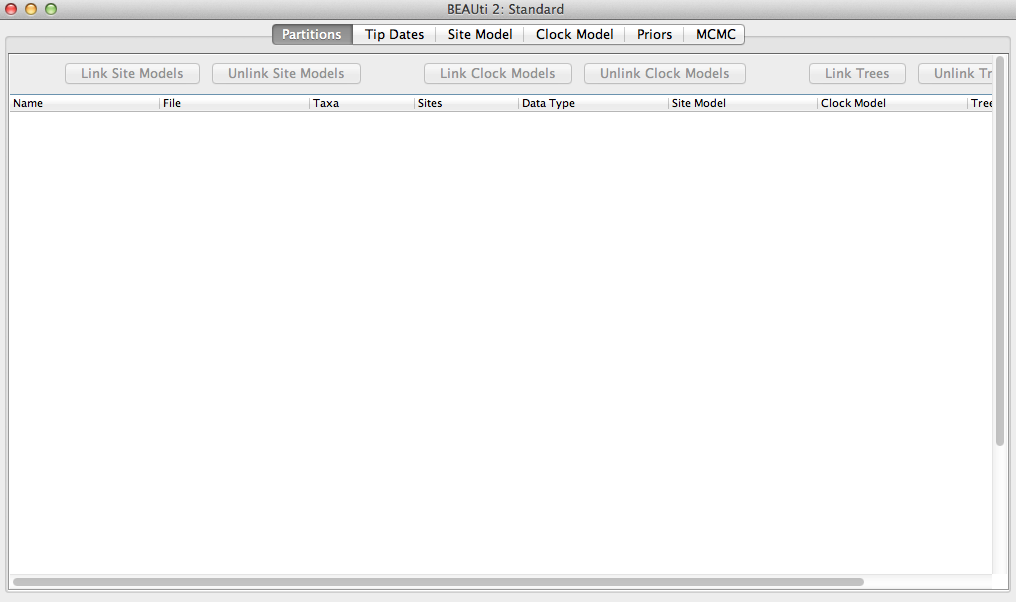
\includegraphics[width=0.7\textwidth]{screenshots/beauti-init.png}}
        \caption{BEAUTi window launched from \texttt{BEAST}.}
        \label{fig:beautiInit}
    \end{figure}
}

\step{Install SNAPP and model selection packages}{You need to add functionality to \texttt{BEAST} in order to estimate 
     species trees with SNP data and 
     to perform model selection. Begin by using the drop-down 
     menu \subItem{File}{Manage Packages.} A window should 
     appear that looks something like Figure~\ref{fig:beauti-manage-packages}.
     Select and install the packages \texttt{{\bf SNAPP}} and \texttt{{\bf Model\_Selection}}. You can then exit the 
     window by clicking the {\bf ``Close''} button.
    \begin{figure}[htbp]
        \centering
        \fbox{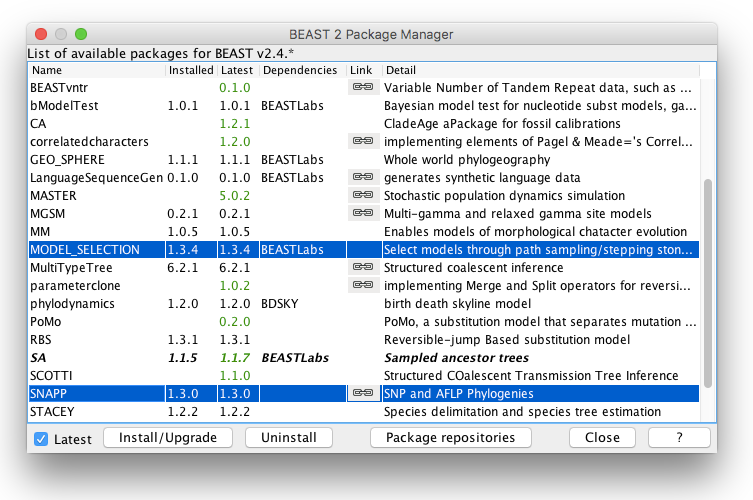
\includegraphics[width=0.7\textwidth]{screenshots/beauti-manage-packages.png}}
        \caption{\texttt{BEAUTi} package manager for \texttt{BEAST}.}
        \label{fig:beauti-manage-packages}
    \end{figure}

}

\step{Converting \texttt{BEAUTi} to \texttt{SNAPP} mode}{Tell \texttt{BEAUTi} that you are  
     setting up a \texttt{SNAPP} analysis, which will change the menu options and allow us to import SNP data.
     Begin by using the drop-down 
     menu \subItem{File}{Template, SNAPP.} 
     This should change the appearance of the \texttt{BEAUTi} 
     window to look something like Figure~\ref{fig:beauti-snapp}.

    \begin{figure}[htbp]
        \centering
        \fbox{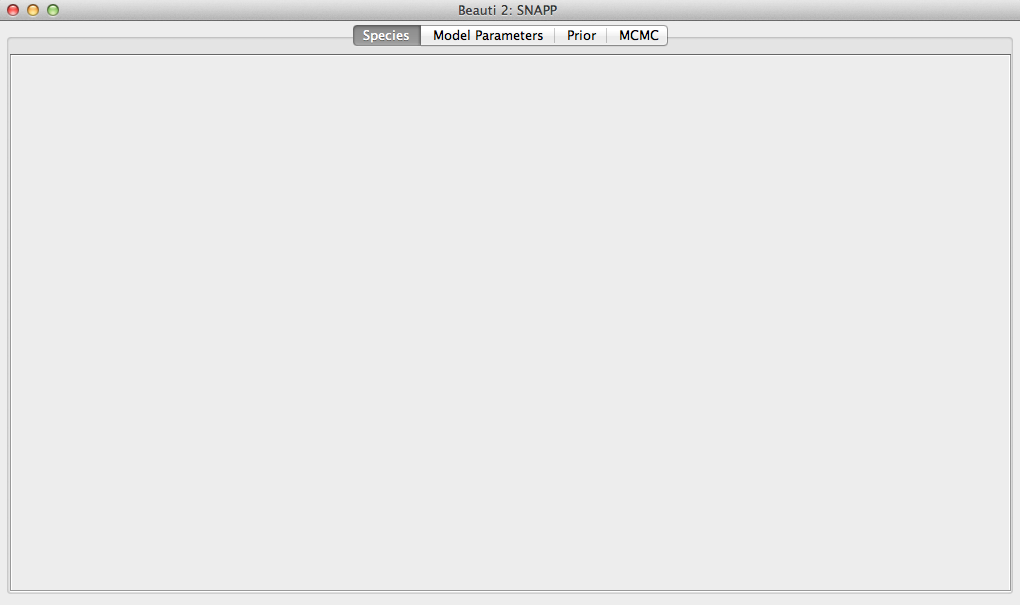
\includegraphics[width=0.7\textwidth]{screenshots/beauti-snapp.png}}
        \caption{\texttt{BEAUTi} window after importing the \texttt{SNAPP} template. Notice that the menu tabs have changed.}
        \label{fig:beauti-snapp}
    \end{figure}

}


\step{Import the SNP data.}{
    Import the SNP data (the {\bf smallhemi129.nex} file)
    using the drop-down menu \subItem{File}{Import Alignment} or \subItem{File}{Add Alignment} (the exact name depends on your operating system).
    Once the data are successfully loaded into \texttt{BEAUTi} you should see a list of the 
    samples included in the data file (Figure~\ref{fig:beauti-data-imported}.)

    \fbox{
    \centering
    \parbox[b][13em][c]{\textwidth}{Figure~\ref{fig:beauti-data-imported} shows the complete set of samples if you load the full data set from {\bf hemi129.nex}, but we recommend loading the small data set file {\bf smallhemi129.nex} because otherwise you might not finish this tutorial in the allocated time frame. In a real analysis, how many samples should you include? The number of samples slows down SNAPP much more than the number of SNPs. Therefore, if your analyses are going too slow, then it is typically better to randomly subsample down to an even proportion of sequences from each species instead of removing SNPs. Reducing the number of samples by half will more than halve the analysis time. When setting up a new analysis, start with a small number of samples for each species (for example, 4 samples per species), which will enable you to make quicker progress. Increase the number of samples once your analyses are returning reasonable results. If you are overambitious with your sampling, then your analyses will become unbearably slow.}
    }

    \begin{figure}[htbp]
        \centering
        \fbox{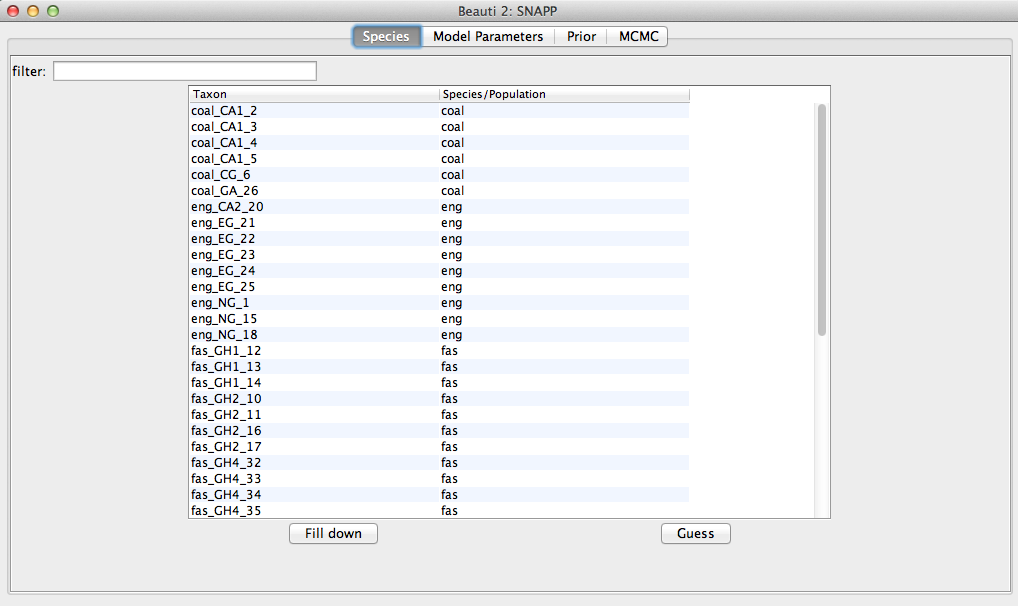
\includegraphics[width=0.8\textwidth]{screenshots/beauti-data-imported.png}}
        \caption{The data successfully loaded by BEAUTi.}
        \label{fig:beauti-data-imported}
    \end{figure}
}

\step{Define species.}{
    There are several ways to designate species assignments. You can automatically 
    designate species names using the names already 
    present in the data files. The species names can be pre-defined this way by including a ``delimiter'' that 
    allows the species name to be parsed from the rest of the sequence name. The gecko data 
    file uses an underscore ``\_'' to separate
    the species name (on the left) from the rest of the sequence name (on the right) as follows:\\
    \\
    \cmd{eng\_NG\_1}\\ 	
    \cmd{coal\_CA1\_2}\\	
    \cmd{coal\_CA1\_3}\\
    \cmd{coal\_CA1\_4}\\	
    \cmd{coal\_CA1\_5}\\	
    \cmd{coal\_CG\_6}\\	
    \cmd{kya\_GH3\_7}\\	
    \cmd{kya\_GH3\_8}\\	
    \cmd{\ldots}\\
    \\
    Several options for assigning species names are available using the ``Guess'' button. The screen should look similar to 
     Figure~\ref{fig:beauti-guess-trait}. You can even import a custom mapping file that links each sample to a species using the ``read from file'' option.    
     
    \begin{figure}[htbp]
        \centering
        \fbox{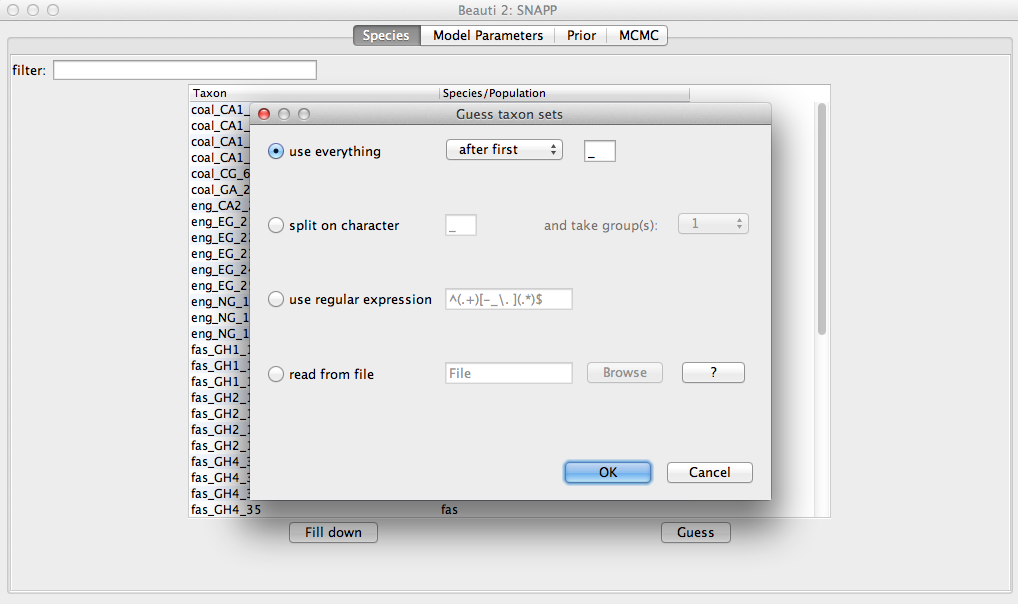
\includegraphics[width=0.8\textwidth]{screenshots/beauti-guess-trait.png}}
        \caption{The species assignment options that appears after you select the ``Guess' button.}
        \label{fig:beauti-guess-trait}
    \end{figure}

    To extract the species names in this tutorial, keep ``use everything'' selected and leave the underscore in the text box,
    but change ``after first'' to {\bf ``before first''}.
    Click the ``Ok'' button to return to the \menutab{Species} window. Be sure that each Taxon has a Species/Population name.    
}


\step{Set the mutation model.}{
    Next, set up our model under the \menutab{Mutation Parameters} tab (Figure~\ref{fig:beauti-mutation}).
    Be sure to read the documentation \href{http://www.beast2.org/tutorials}{A rough guide to \texttt{SNAPP}} to learn more about the model options. Briefly, the parameters are as follows:

\small{
    \begin{compactdesc}
       \item[\field{Mutation Rate U: instantaneous rate of mutating from the 0 allele to the 1 allele.}]
       \item[\field{Mutation Rate V: instantaneous rate of mutating from the 1 allele to the 0 allele.}]
       \item[\field{Coalescence Rate: population size parameter with one value for each node in the tree.}]
    \end{compactdesc}
    
    \textit{Recommendations:}  Set mutation rates u and v = 1, and disable sampling by unchecking the ``Sample'' box adjacent to the u parameter. For SNP data where the ``0'' and ``1'' alleles are arbitrarily assigned from the data, it usually makes no sense to uncouple these rates.

    Alternatively -- if you know what you are doing! -- you can click the {\bf ``Calc mutation rates''} button to get a direct estimate of u and v. Either way, you typically do not have to estimate these parameters during the MCMC. 
    Coalescent Rate: make sure the Sample box is ticked so that MCMC sampling of this parameter is enabled. If you do not sample, then you assume that all population sizes are the same, which is unrealistic. The coalescent rate is 2/theta, and the number is simply the starting value used to initialize the analysis. Do not confuse the coalescent rate with the theta prior. The theta prior is described in detail in the next section.
    
    The ``Include non-polymorphic'' checkbox is used in cases where invariant sites have been included in the data. The likelihood calculations are 
    different if \texttt{SNAPP} assumes that all constant sites have been removed. The example dataset for this tutorial, like typical SNP datasets, only includes variable site so make sure that the box is not checked.
    
    The ``Mutation Only At Root'' checkbox indicates conditioning on zero mutations, except at root (default false). As a result, all gene 
    trees will coalesce in the root only, and never in any of the branches. This option allows you to emulate the model used by \citet{nielsen1998} and \citet{roychoudhury2008}.
    
    The ``Show Pattern Likelihoods And Quit'' checkbox is handy if you just want to print out the likelihoods for all patterns in the starting state and then quit.
    
    The ``Use Log Likelihood Correction'' checkbox is for calculating corrected likelihood values for Bayes factor test of different species assignments (the calculation is almost instantaneous, and it will not slow down your analysis).
    This is a species assignment and delimitation tutorial so make sure this box is checked!

    Unless things break, leave ``Use Tip Likelihoods'' and ``Implementation'' at their default settings.

    }
    
        \begin{figure}[htbp]
        \centering
        \fbox{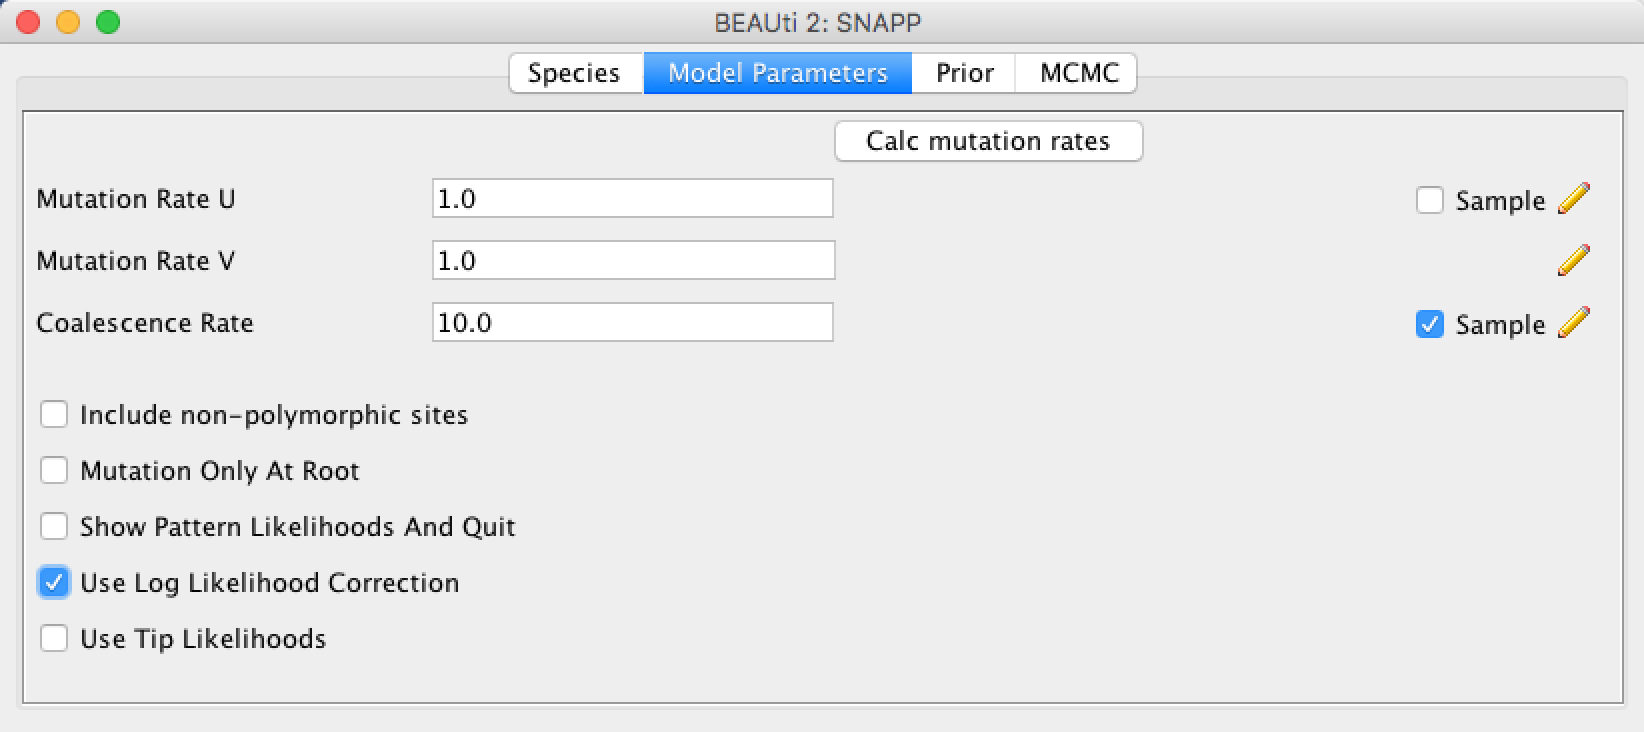
\includegraphics[width=0.8\textwidth]{screenshots/beauti-mutation.png}}
        \caption{The Mutation Parameters options.}
        \label{fig:beauti-mutation}
    \end{figure}
}

    
\step{Define the priors.}{
    Next, move to the \menutab{Prior} tab to specify the priors. Again, read the 
    documentation \href{http://www.beast2.org/tutorials}{A rough guide to \texttt{SNAPP}} 
    to learn more about these priors. It is important to be aware of the biological meaning of these priors. 
    One problem with \texttt{SNAPP} is that it is deceptively easy to set up an analysis using default options,
    but those defaults are almost certainly inappropriate for your particular study.

    Lambda (or $\lambda$) refers to the speciation rate in the Yule model. The default prior on lambda of 1/X is uninformative and improper. This is not necessarily
    bad if you truly have no prior knowledge of what this rate should be. However, improper priors \textbf{cannot} be used for Bayes factor analyses, and so must be changed for this tutorial.
    Species of the genus \textit{Hemidactylus} seem to bifurcate every 0.0025 substitutions per site or so, so change the prior on lambda to a Gamma distribution, and set the beta scale parameter to 200.
    This corresponds to a mean of 400, or 400 speciation events for every substitution per site of tree length (Figure~\ref{fig:beauti-prior2}). The alpha shape parameter of 2 corresponds to a modal but broad distribution, so we are not letting
    this prior swamp the signal present in the data. Change the initial value of lambda---under ``snapprior''---to a more realistic initial value like 10. The initial value won't change your results, but it may speed up the MCMC a little.

    \begin{figure}[htbp]
        \centering
        \fbox{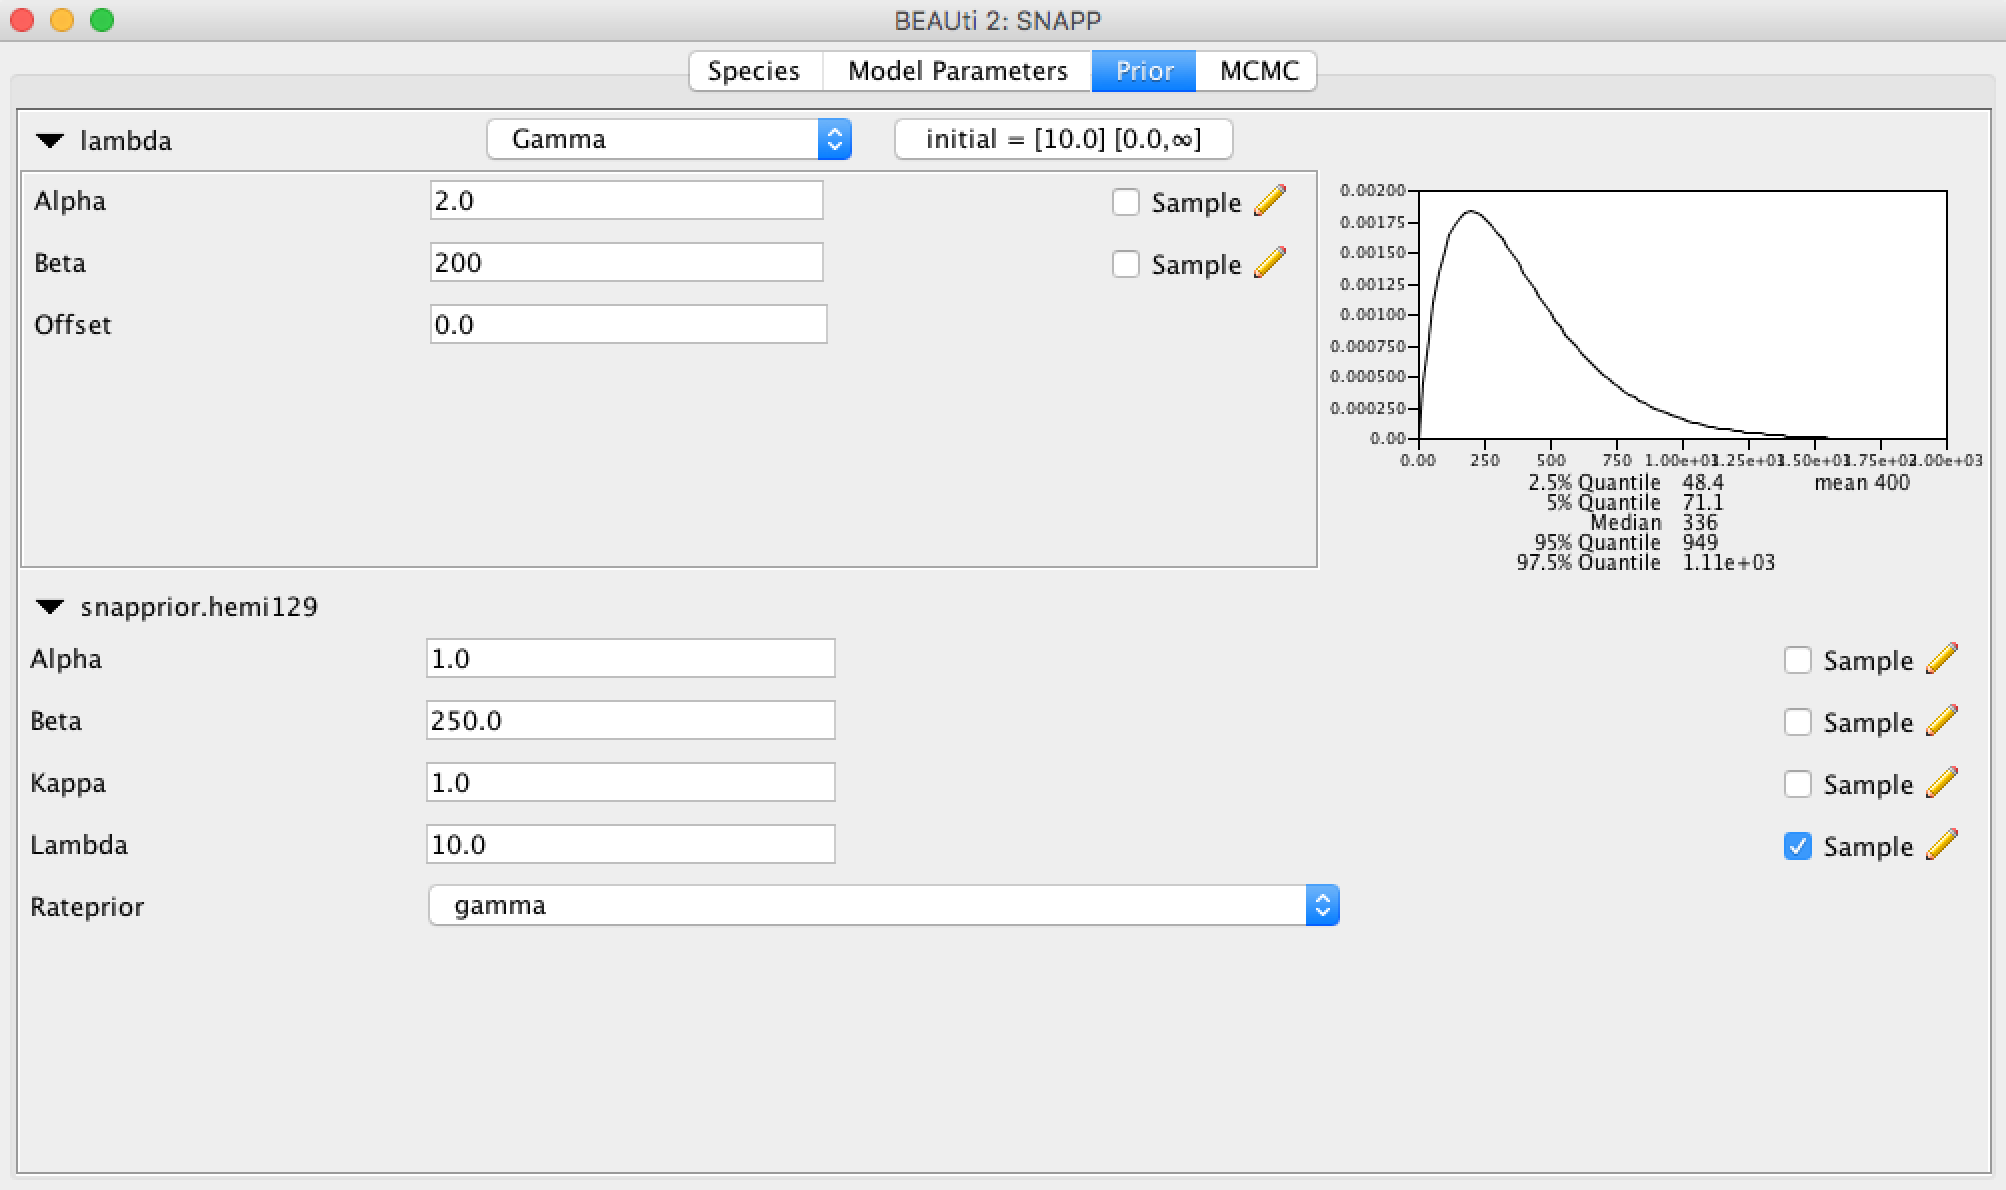
\includegraphics[width=0.8\textwidth]{screenshots/beauti-prior2.png}}
        \caption{Using a gamma prior for Lambda.}
        \label{fig:beauti-prior2}
    \end{figure}

    Rateprior sets the prior distribution used for theta. Recall that for a
    diploid population, theta = 4Nu, where N is the effective population size
    and u is the per-generation mutation rate. If theta=0.004, you expect to
    observe 0.4\% variation between two randomly sampled alleles in a
    population. Another way to think about this is in the expected number of
    substitutions; ``theta=0.004'' means that for two randomly sampled
    phased sequences within a population you expect to observe 4 SNPs in 1,000
    bases.

    The ``snapprior'' parameters alpha, beta and kappa are contextually
    dependant on the distribution chosen for Rateprior. Using the default
    gamma distribution the kappa paremeter is
    ignored, and the alpha and beta parameters correspond to the shape
    and \textit{rate} of the distribution (rather than the default shape and
    \textit{scale} used elsewhere in BEAUTi). When using a gamma distribution
    here, the mean of the prior on theta will therefore be alpha $\div$ beta.

    For this tutorial, set alpha to 1 and beta to 250. This corresponds to
    a decaying distribution with a mean of 0.004, or an expectation of 4 heterozygous sites per 1,000 bases, a
    reasonable value for the data set in this tutorial. As with the speciation
    rate, the posterior values of theta will be strongly influenced by the data.
}

\step{Specify MCMC settings and generate the XML file.}{
    Next, move to the \menutab{MCMC} tab. 
    Change the following settings:
    \begin{compactdesc}
        \item[\field{Chain Length:}] \fieldvalue{1000}
        \item[\field{Store Every:}] \fieldvalue{10}
        \item[\field{tracelog:File Name:}] \fieldvalue{RunA.log}
        \item[\field{tracelog:Log Every:}] \fieldvalue{10}
        \item[\field{screenlog:Log Every:}] \fieldvalue{10}
        \item[\field{treelog:File Name:}] \fieldvalue{RunA.trees}
        \item[\field{treelog:Log Every:}] \fieldvalue{10}
    \end{compactdesc}
    Leave the remaining options at their default values
    (Figure~\ref{fig:beauti-mcmc}). These MCMC values are way to low, and a thorough analysis requires much more computational time. 
    The MCMC run times are intentionally kept short (and the data files reduced) in this tutorial. These short analyses should run in approximately 2 -- 4 minutes depending
    on the number of processors available on your computer.  
    Thorough analyses of the full data takes 2 -- 6 days, depending on the number of species in the model, and generally require at least 100,000 generations. Running multiple independent chains using different starting seeds and comparing results is a good way to ensure that the analyses are converging.
 
    \begin{figure}[htbp]
        \centering
        \fbox{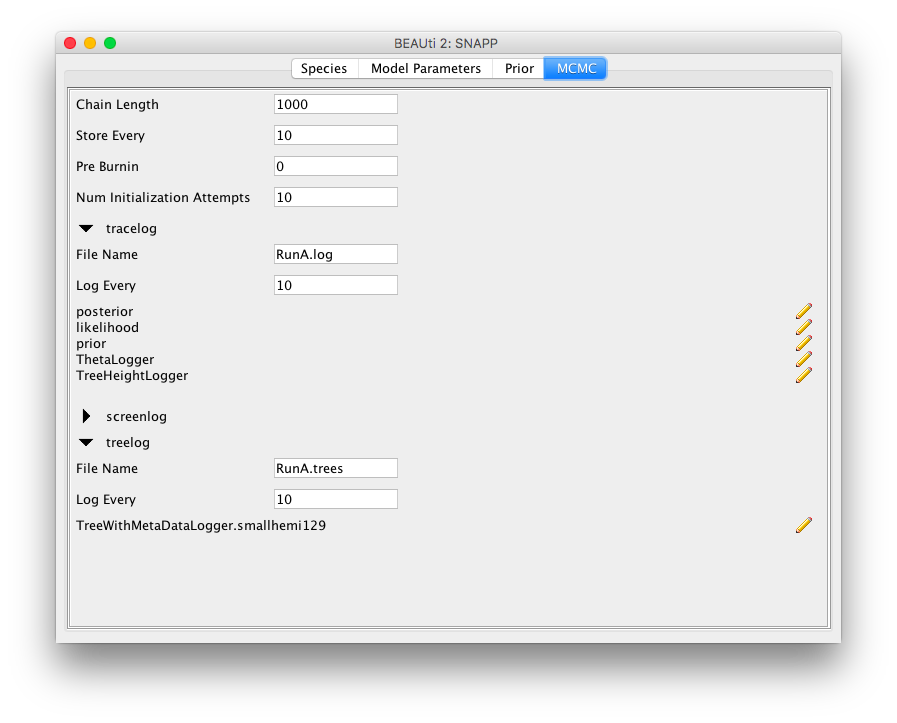
\includegraphics[width=1.0\textwidth]{screenshots/beauti-mcmc.png}}
        \caption{The MCMC settings.}
        \label{fig:beauti-mcmc}
    \end{figure}

    Next, save the file using \subItem{File}{Save\ldots.} 
    Another subwindow will appear for specifying the name and location for
    saving the XML file. Name the file ``RunA.xml'' and place it in a new folder called ``RunA'' you may create in the ``BFD'' tutorial folder.\\
    }

\intermediate{\subsection{Running the stepping stone analysis with \texttt{BEAST}}}

\step{Setting up for marginal likelihood estimation.}{
There are two ways to set up the stepping stone analysis; through a GUI, and by editing the XML. The GUI is more convenient but makes it a bit harder to transfer the analysis to a cluster, and since stepping stone analyses are typically very computational intensive, it often makes sense to run them on a cluster. In this step, we explain how to set up the analysis using the GUI, and in the next two steps it is explained how to set up an XML file through a text editor.

First, start the BEAST app-store by selecting the File/Launch apps menu in BEAUti (alternatively, double click the AppStore icon in the BEAST folder). A window similar to Figure~\ref{fig:appstore} should pop up.

    \begin{figure}[htbp]
        \centering
        {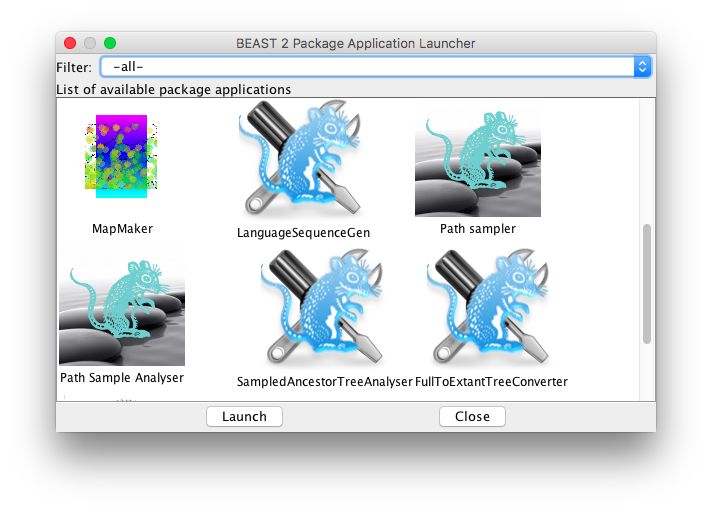
\includegraphics[width=0.6\textwidth]{screenshots/appstore}}
        \caption{BEAST app store.}
        \label{fig:appstore}
    \end{figure}

Select the Path sampler icon, and hit the Launch button. A new window pops up with the GUI for path sampling/stepping stone analysis similar to Figure~\ref{fig:pathsampler}. 

If you prefer to start from the command line, you can use the following in a terminal:

    	    \cmd{/path/to/beast/bin/appstore PathSampler}

We need to change some of the settings for this tutorial:

    \begin{compactdesc}
       \item[Model1:]{Use the browse button to select the file with MCMC analysis you just set up in BEAUti.}
       \item[Alpha:]{Changing this can help -- or hurt -- the efficiency of the numerical integration of the marginal likelihood, leave at the default.}
       \item[Nr Of Steps:]{The number of steps to use, more is better but slower. Change to 12.}
       \item[rootdir:]{Folder for storing output. Change to the \textbf{full} path of the ``RunA'' folder you created earlier. For example, on my computer this is ``/home/me/Documents/beast-docs/BFD/RunA'' (without the quote marks).}
       \item[Chain Length:]{The length of each chain for each step. Change it to 1000. Longer is better, but 1000 steps will fit within the tutorial time.}
       \item[Burn In Percentage:]{Burn-In percentage used for analyzing the log files, leave at the default.}
       \item[Pre Burnin:]{Number of samples that are discarded for the first step, but not the others. Change to 0.}
       \item[Do Not Run:]{Create the necessary XML files and exit, useful for running on clusters. Leave off.}
       \item[Delete Old Logs:]{Delete any previously created log files. Leave off.}
    \end{compactdesc}

    \begin{figure}[htbp]
        \centering
        {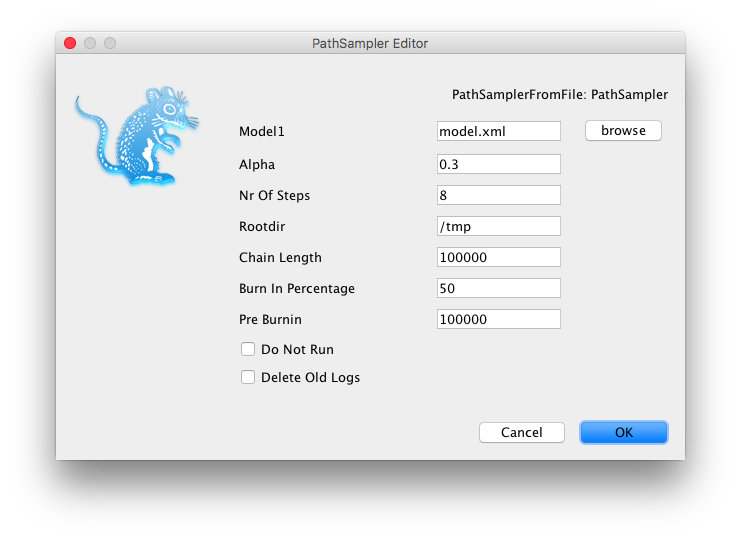
\includegraphics[width=0.7\textwidth]{screenshots/pathsampler}}
        \caption{GUI for path sampling/stepping stone analysis.}
        \label{fig:pathsampler}
    \end{figure}

Now just click OK to run the stepping stone sampling for the ``RunA'' species delimitation hypothesis.

{\bf Step 11b}. Manually editing the XML file for marginal likelihood estimation -- OPTIONAL and ALTERNATIVE to Step 11. Instructions for setting up
marginal likelihood estimation using path/stepping stone sampling are provided at the \href{http://www.beast2.org/path-sampling/}{BEAST} website. The procedure involves (1) typing in some short codes in a few places, (2) replacing some words, and (3) copying and pasting some sections around. Specific instructions are below:
 
Open your XML file in a text editor. Search and replace the opening run statement (located about half way through the file) with an mcmc statement by changing {\bf ``<run ...>''} into {\bf ``<mcmc ...>''.} Next, type a new closing mcmc statement, {\bf ``</mcmc>''}, just before the closing run statement, {\bf ``</run>''}, located at the end of the file.

Now you are ready to insert the path/stepping stone sampling commands. You will need to insert the following block of text into your XML file immediately above the opening ``<mcmc ...>''' element:

\texttt{
<run spec=\textquotesingle beast.inference.PathSampler\textquotesingle \\
chainLength=\textquotedbl 1000\textquotedbl\\
alpha=\textquotesingle 0.3\textquotesingle \\
rootdir=\textquotesingle /path/to/BFD/RunA/\textquotesingle \\
burnInPercentage=\textquotesingle 50\textquotesingle \\
preBurnin=\textquotedbl 0\textquotedbl\\
deleteOldLogs=\textquotesingle true\textquotesingle \\
nrOfSteps=\textquotesingle 12\textquotesingle >\\
cd \$(dir)\\
java -cp \$(java.class.path) beast.app.beastapp.BeastMain \$(resume/overwrite) -java -seed \$(seed) beast.xml\\
}

{\bf Important:} If you copy and paste this section into your XML file, be sure to check that the symbols paste correctly. Also, make sure that the root folder path (rootdir) exists on your computer.

	These path sampling parameters are way to low, and a thorough analysis requires much more computational time. Stable marginal likelihood estimates usually require at least 48 steps (sometimes 100), chainLength = 100,000 (sometimes 1,000,000), and preBurnin=10,000 (sometimes 100,000). The MCMC run times are 
    intentionally kept short in this tutorial to obtain quick (but meaningless) results. The run time on a MacBook Pro 2.3GHz i7 processor with 16GB of memory is approximately 2.5 minutes, and this is running 8 concurrent steps (= 8 threads). Increasing the number of threads will speed up the analysis by running more concurrent path sampling steps, but this requires more memory (this analysis uses about 12GB of memory). For large-scale analyses, many users find that they run out of memory before processors.

The path sampling parameters that you just entered into your XML file are as follows:

    \begin{compactdesc}
       \item[chainLength:]{MCMC sample length for each path sampling step.}
       \item[alpha:]{parameter used to space out path sampling steps.}
       \item[rootdir:]{folder for storing output. Be sure that the folder exists before starting the run.}
       \item[burnInPercentage:]{burn-In percentage used for analyzing the log files.}
       \item[preBurnin:]{number of samples that are discarded for the first step, but not the others.}
       \item[deleteOldLogs:]{delete existing log files from rootdir}
       \item[nrOfSteps:]{the number of path sampling steps to use}
    \end{compactdesc}

	    You can execute the XML file in \texttt{BEAST} using the GUI or the command line. If you are using Mac OS or Windows, you should 
	    be able to launch the \texttt{BEAST} GUI by double clicking on the application icon. 
	    After the \texttt{BEAST} window appears, click the \field{Choose File\ldots} button, 
	    and select the XML file you just created (Figure~\ref{fig:beast}). Increase the \field{Thread pool size} to speed up your analysis. 
	    Running SNAPP with multiple threads can increase speeds, but experimenting with the number of threads is required to get the best performance.

	    Click \field{Run}. The analysis should take about 10 minutes. 
	    You can also run \texttt{BEAST} from the command line. Open the {\bf Terminal} Application and navigate to the ``RunA'' folder. To execute the file, type the following at the command line:
	    
	    \cmd{/path/to/beast/bin/beast -threads 8 RunA.xml}
	    
	    or
	    
	    \cmd{beast -threads 8 RunA.xml}
	    
	    if you have already copied the \texttt{BEAST} executable to your path. Caution: setting the number of \field{threads} beyond the maximum number available on your computer can have serious drawbacks, and you will probably not have enough memory to support all of those separate analyses.
	  	
	\begin{figure}[htbp]
        \centering
        \fbox{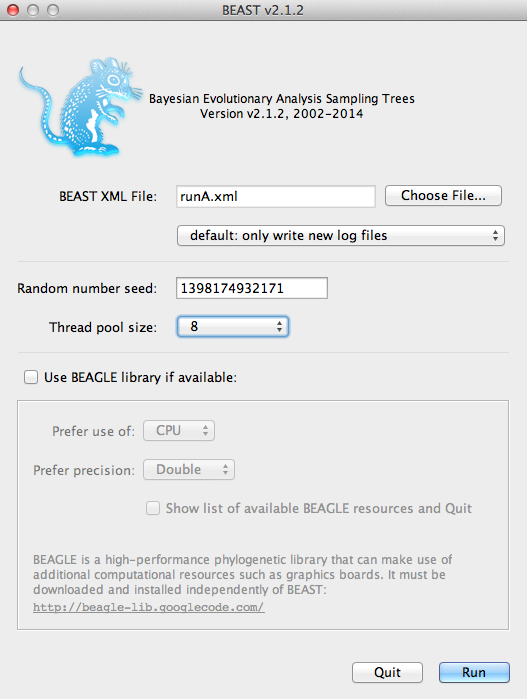
\includegraphics[width=0.5\textwidth]{screenshots/beast.png}}
        \caption{The \texttt{BEAST} GUI window.}
        \label{fig:beast}
    \end{figure}
    }

\intermediate{\subsection{Inspecting path sampling results}}

\step{Inspecting path sampling results.}{
At the end of your analysis, the path sampling results will be displayed on the screen. An example is shown in Figure~\ref{fig:beast-output}. 
Each row shows the results from one path sampling step. The example in Figure~\ref{fig:beast-output} shows the results from a path sampling analysis with 24 steps. You will use the value after ``marginal L estimate'' to compare models. 

       \begin{figure}[htbp]
        \centering
        \fbox{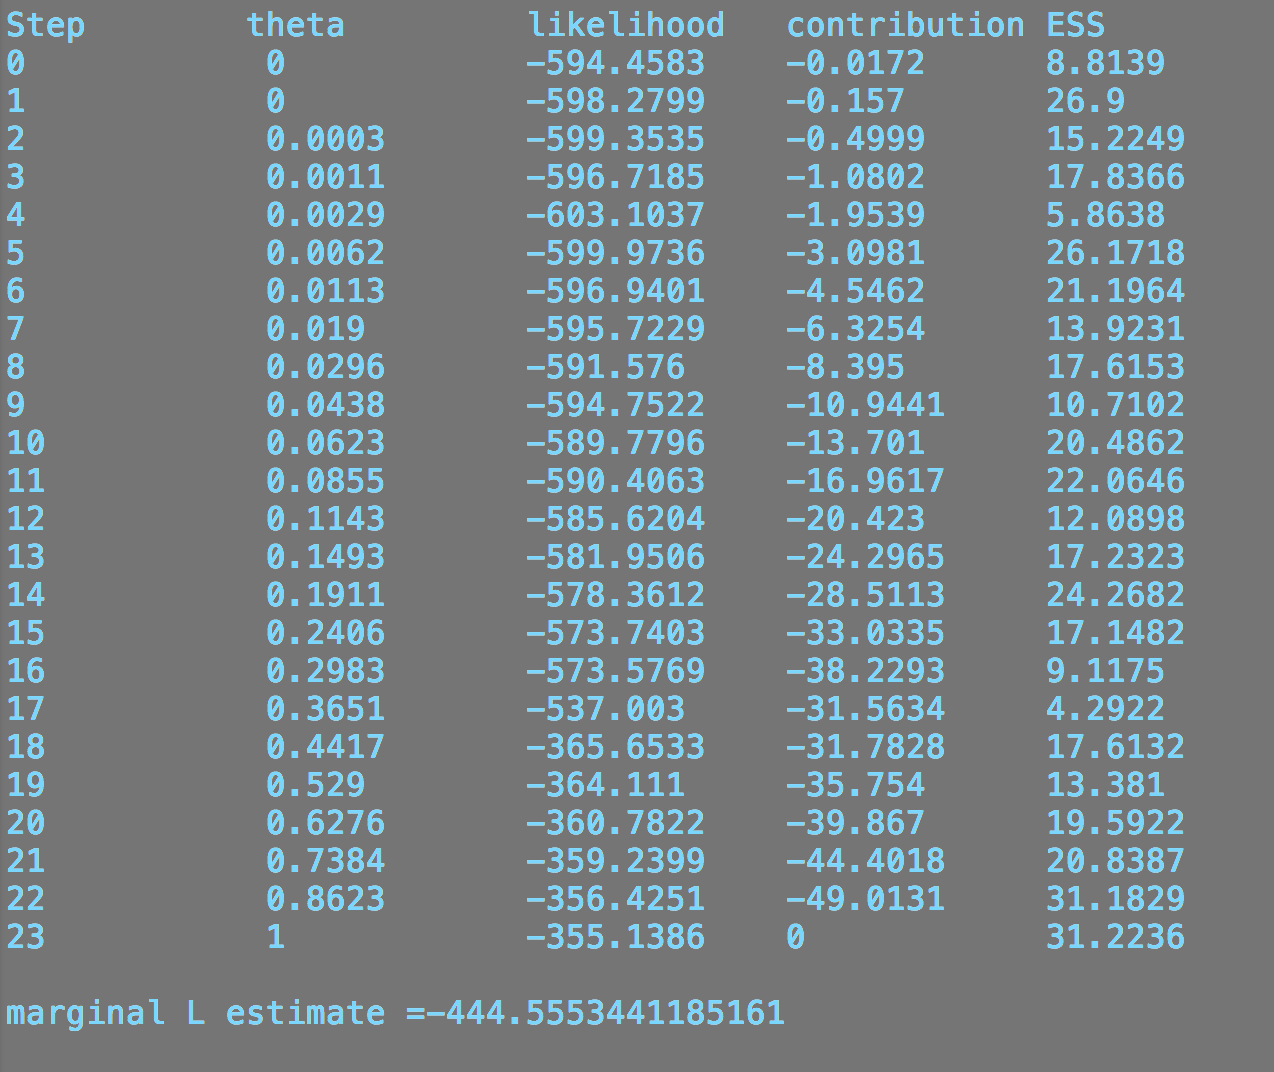
\includegraphics[width=0.5\textwidth]{screenshots/beast-output.png}}
        \caption{The path sampling output at the end of the analysis.}
        \label{fig:beast-output}
    \end{figure}
}



\intermediate{\subsection{Setting up new species delimitation models}}

\step{Setting up new XML files for species delimitation.}{
Now that you have one XML file up and running it is easy to make new XML files for each species delimitation model.
To prepare a new file for species delimitation, make a few slight modifications to the existing RunA.xml file: (1) save a copy of the xml file as RunB.xml and save it in a new folder called ``RunB'', (2) find and replace ``RunA'' with ``RunB'' in the xml file so that you don't accidentally overwrite any of your previous results, (3) change the species assignments.

This last part requires changing the number and/or composition of taxonset features. Each taxonset begins with {\bf ``<taxonset ...>''} and ends with {\bf ``</taxonset>''} (Figure~\ref{fig:beast-taxon-set}). To lump species, simply combine the taxon names into a single taxonset feature. To split a species, simple create a new taxonset with an appropriate new ``id'' name, and cut and paste the relevant \textbf{``<taxon ... />''} elements. To reassign a taxon to another species you can cut and paste the taxon to a different taxonset. 
Although you could create a new XML with the alternative species assignments from scratch by rerunning \texttt{BEAUTi}, it is much more efficient to duplicate your already existing XML and edit the taxonsets.

       \begin{figure}[htbp]
        \centering
        \fbox{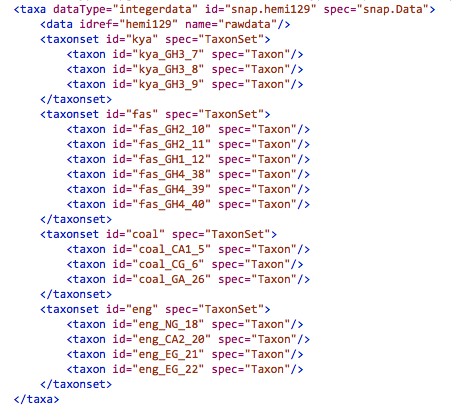
\includegraphics[width=0.5\textwidth]{screenshots/beast-taxon-set.png}}
        \caption{Example of the taxonset features in the XML file.}
        \label{fig:beast-taxon-set}
    \end{figure}

While the taxon names in the data and XML files are a little cryptic, it
should be straightforward to lump species based on the hypotheses in
Figure~\ref{fig:map}. For splitting and reassignment, you should transfer the
following individuals:

\begin{compactdesc}
    \item[H. fasciatus:]{Split (RunE) Ankasa Conversation Area samples, labeled as fas\_GH4\_38, \_39 and \_40.}
    \item[H. eniangii:]{Split (RunF) or reassign (RunG) Bioko Island individuals, labeled as eng\_EG\_21 and \_22.}
\end{compactdesc}

After you have set up an XML file for each hypothesis you can calculate the marginal likelihoods by running through Step 11 again for each XML individually.
}

\step{Comparing species delimitation models with Bayes factors.}{  
   After you run each of the alternative species delimitation models you can rank them by their marginal likelihood estimate (MLE). You 
   can also calculate Bayes factors to compare the models. 
   The Bayes factor (BF) is a model selection tool that is simple and well suited for the purposes of comparing species delimitation models. 
   Calculating the BF between models is simple. To do so, simply subtract the MLE values for two models, and then multiply the difference by two:

   \begin{equation}
   \text{BF} = 2 \times (\text{MLE}_1 - \text{MLE}_0)
   \end{equation}

   A positive BF value indicates support in favor of model 1, while a negative BF value indicates support in favor of model 0. To calculate Bayes factors in this tutorial, the current taxonomy (RunA) will always be model 0.

The strength of support from BF comparisons of competing models can be evaluated using the framework of \cite{kass95}. 
 The BF scale is as follows: 
0 < BF < 2 is not worth more than a bare mention, 2 < BF < 6 is positive evidence, 6 < BF < 10 is strong support, and BF > 10 is decisive.

The results for the seven gecko models are provided in Table 2. The model that splits \textit{eniangii} into two species (RunF) is the top-ranked model. It has the highest MLE value, and it is supported in favor of the current taxonomy model (RunA). The BF in support for model F is decisive compared to model A. It is important to emphasize that these results are \textit{tragically deficient} in terms of the MCMC analysis. Much, much longer runs are required to obtain stable results. 

Table 2: Stepping stone sampling results for the seven species delimitation models shown in Figure \ref{fig:map}. Positive BF values indicate support for the alternative model, and negative BF values indicate support for the current taxonomy.
\begin{table}[ht]
\tabcolsep=0.2cm
\begin{tabular}{l c c c c } 
\hline     
Model 							& Species 	& MLE 	& Rank 		& BF\\
\hline
RunA, current taxonomy & 4 & -816.41 & 2 & --.--\\
RunB, lump western forests & 3 & -846.21 & 5 & -59.60\\
RunC, lump central forests & 3 & -883.16 & 6 & -133.50\\
RunD, lump western and central forests & 2 & -899.22 & 7 & -165.62\\
RunE, split \textit{fasciatus} & 5 & -840.17 & 4 & -47.52\\
RunF, split \textit{eniangii} & 5 & -766.03 & 1 & 100.76\\
RunG, reassign Bioko Island & 4 & -818.87 & 3 & -4.92\\
\hline
\end{tabular}\\
MLE = Marginal likelihood estimate\\
BF = Bayes factor\\
\end{table}
}

\intermediate{\subsection{Summarizing the trees using \texttt{TreeAnnotator}.}}

\step{Summarize the species tree using \texttt{TreeAnnotator}.}{
TreeAnnotator will summarize the posterior distribution of species trees and identify the topology with the best posterior support, and summarize the divergence times for each node in the tree.
	Launch the \texttt{TreeAnnotator} program.
	For the \field{Target tree type} field, choose \fieldvalue{Maximum clade credibility tree}.
    For the \field{Node heights} field, choose \fieldvalue{Median heights}.
	You will typically only want to summarize the results corresponding to theta=1, which is the step where trees are sampled from the posterior distribution. Check the SNAPP screen output to verify which path sampling step corresponds to theta=1 (this changes with different versions of SNAPP). Select the \field{Input Tree File} button and select the file ``RunA.trees'' in the stepN subfolder of ``RunA'' that corresponds to theta=1.
	Select the \field{Output File} button to specify the output folder and a file name, e.g. ``RunA-MCC.tree''.
	Click \field{Run}
}

\intermediate{\subsection{Visualizing the tree in \texttt{FigTree}}}

\step{Visualize the species tree in \texttt{FigTree}.}{
    Launch the \texttt{FigTree} program, and load the ``RunA-MCC.tree'' file
    you just created with \texttt{TreeAnnotator}.
    Check the \field{Branch Labels} option and select
    \fieldvalue{posterior} for the \subItem{Branch labels}{Display} fields.
    Check the \field{Node Bars} option and select
    \fieldvalue{height\_95\%\_HPD} for the \subItem{Node bars}{Display} field.
 
 
 You can also get a summary of some tree statistics using the TreeSetAnalyser, which you can launch from the BEAST app launcher, and looks something like Figure~\ref{fig:treesetanalyser}
       \begin{figure}[htbp]
        \centering
        \fbox{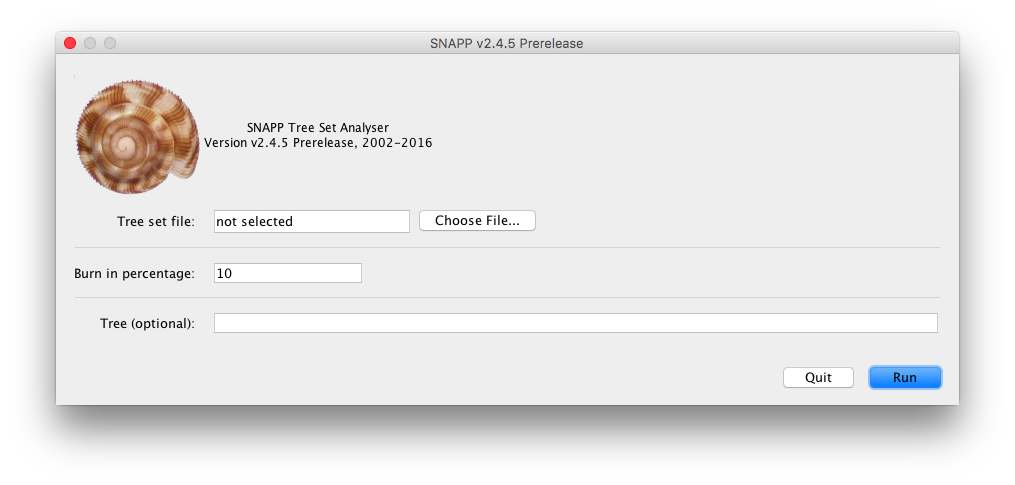
\includegraphics[width=0.5\textwidth]{screenshots/treesetanalyser.png}}
        \caption{Tree set analyser utility.}
        \label{fig:treesetanalyser}
    \end{figure}
     }




